\documentclass[a4paper,12pt]{report}
\usepackage{graphicx}
\title{Tugas pemrograman Chapter 4}
\author{Nuha Hanifatul Khonsa'}
\date{1 Desember 2019}
\begin{document}


\maketitle

\section{Pemahaman Teori}
\begin{enumerate}
    \item CSV, Pengertian, Fungsi dan Contoh File
    \begin{itemize}
        \item Pengertian
        \par CSV atau comma separated value ialah salah satu tipe file yang dapat digunakan dalam dunia programming. File CSV sendiri sering digunakan dalam pengolahan informasi yang dihasilkan spreadsheet untuk diproses lebih lanjut melalui mesin analitik.CSV menggunakan format file/data pada tiap record dipisahkan menggunakan koma(,) ataupun tabda titik (.). File CSV dapat dijumpai pada notepad, excel, wordpad.
        \item Fungsi
        \par CSV berfungsi dalam memudahkan pemindahan data dari satu program ke program lain.
        \item Contoh File CSV
        \par\textit{NPM,nama, kelas}
        \par\textbf{1184085,Nuha Hanifatul Khonsa',D4TI2C}
        \par\textbf{1184095, Dian Markuci, D4TI2C}
    \end{itemize}
    
    \item Aplikasi yang Dapat Menciptakan File CSV
    \textbf{Aplikasi Editor: Notepad, Wordpad}
    \textbf{Spreadsheet: Microsoft Excel}
    
    \item Cara Menulis dan Membaca File CSV pada Excel(Spreadsheet)
    \begin{enumerate}
        \item Pertama kita dapat membuat dokumen baru pada Microsoft Excel
        \item Lalu kita dapat menambahkan judul kolom pada tiap informasi yang ingin dicatat. Seperti NPM, Nama, Kelas dan isikan sesuai dengan perintah pada judul -> NPM isikan NPM, Nama isikan Nama dari NPM tersebut dan Kelasnya.
        \item yang terakhir kita simpan dalam format .CSV
    \end{enumerate}
    
    \item Sejarah Library CSV
    \par Library CSV sering digunakan untuk merepresentasikan sebuah data. Format ini termasuk dalam standar file ASCII. File CSV digunakan untuk menyimpan informasi yang dipisahkan oleh koma, bukan menyimpan informasi dalam kolom.Dan jika teks dan angka disimpan dalam bentuk csv maka mudah untuk memindahkannya dari satu program ke program lain. 
    
    \item Sejarah Library Pandas
    \par Pandas adalah librari analisis data yang memiliki struktur data untuk membersihkan data mentah ke dalam sebuah bentuk yang cocok untuk analisis (yaitu tabel). Selain itu, Pandas melakukan tugas penting seperti menyelaraskan data untuk perbandingan dan penggabungan set data, penanganan data yang hilang, dll, Nah, awal mulanya pandas didesain untuk menangani data finansial, dikarenakan altenatif umum adalah menggunakan spreadsheet (seperti pada Microsoft Excel).
    
\end{enumerate}
\begin{itemize}
    \item \textbf{Contoh Pemanggilan File .cvs}
    \begin{center}
    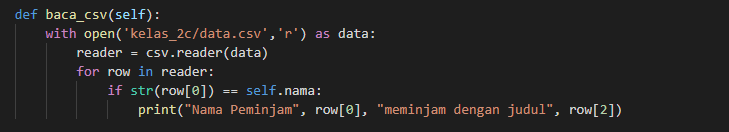
\includegraphics[width=11cm\textwidth]{figure/baca.png}
    \end{center}
    \item \textbf{Contoh Library Pandas}
    \begin{verbatim}
        import pandas
        df=pandas.read_csv('data.csv')
        df.to_csv('data.csv')
    \end{verbatim}
\end{itemize}



\end{document}
